
% TODO: "probing" a matrix with each of the basis vectors is enough to
% completely characterize the matrix.

\chapter{Matrices}

It's now time for the granddaddy of all linear algebra entities: the
\textbf{matrix}. When we've finished this part of our climb, you'll actually be
able to see the summit we'll eventually reach.

By the way, the plural of \textit{matrix} is \textbf{matrices} (pronounced
MAY-trih-sees), kind of like the plural of \textit{index} is \textit{indices.}
But don't forget the singular is still ``\textit{matrix}!'' Don't let me (or
anyone else) catch you uttering the non-word ``matrice'' -- you'll sound like a
dweeb and drive me up a wall.

\section{Row and column vectors}
\index{vector}

Up to now, a vector has simply been a vector. I haven't made a big deal about
how you write it on the page. We've been free to write a vector
$\overrightarrow{\textbf{x}}$ with the three elements 6, 2, and 9 in either of
these ways:

\vspace{-.15in}
\begin{center}
\begin{tabular}{ccc}
$\overrightarrow{\textbf{x}}$ = \textbf{[}$\ 6\ \ 2\ \ 9\ $\textbf{]} &
\quad\quad \textit{...or...} \quad\quad &
$\overrightarrow{\textbf{x}}$ = $\begin{bmatrix} 6 \\ 2 \\ 9 \end{bmatrix}$ \ 
\end{tabular}
\end{center}
\vspace{-.15in}

\index{function}

Or heck, you could even write it diagonally if you want. This flexibility is
because all that really matters is the \textit{function} view of a vector that
we discussed in section~\ref{vectorIsFunction}. All that ultimately matters is
that you associate the correct index number with the correct element. However I
might draw $\overrightarrow{\textbf{x}}$ on paper, if I asked you for the value
of ``element \#0,'' you'd say 6, and if I asked for ``element \#2,'' you'd say
9. The way it looks has been immaterial up until now.

\index{row vector}
\index{column vector}

That will still be true sometimes. But beginning with this chapter, it's going
to sometimes turn out to matter whether or not we think of a vector as a
\textbf{row vector} (the left-hand-side version of
$\overrightarrow{\textbf{x}}$, above) or a \textbf{column vector} (the
right-hand-side). Memorize these terms: they matter, and you'll have to have
them on the tip of your neural cortex. A row goes horizontally, side-to-side;
and a column goes vertically, up-to-down.

I'll try to always be very careful to emphasize the row vs.~column nature of a
vector in those cases where it turns out to matter.

\index{default}

By the way, one surprising thing (at least, it was to me) is that the
``default'' is for an unspecified vector to be treated as a \textit{column}
vector, not a row. Column vectors take up more room on the page, and aren't as
natural when you're writing on paper, which I guess is why it surprised me. At
any rate, whenever a vector is under discussion, try to visualize it as an
up-and-down column of entries, unless the accompanying text explicitly says
otherwise.

\section{The matrix}

\index{matrix (plural: matrices)}

At last, the matrix. This will seem underwhelming at first, but \textit{boy}
does it pack a wallop.

A matrix is simply a two-dimensional rectangular grid of entries, kind of like
a spreadsheet. We'll use capital letters to designate them, with no special
arrow-like or other adornment. Here's our first example:

\vspace{-.15in}
\begin{align*}
A =
\begin{bmatrix}
5 &-7 &3 &9 \\
18 &4 &1 &1 \\
3 &-3 &\pi &4 \\
\end{bmatrix}
\end{align*}
\vspace{-.15in}

\index{dimension}
\label{dimension}

Matrices are always rectangular, but not always square. The $A$ matrix is
called a ``$3\times 4$'' (three-by-four) matrix, since it has three
\textbf{row}s and four \textbf{column}s. We say that $3\times 4$ are the
matrix's \textbf{dimensions}. Again, it's important to master all this
terminology. When giving the dimensions of a matrix, you always list the number
of rows first, and then the number of columns.

\index{index number}

To specify an individual element, we need \textit{two} indices instead of just
one as we did for a vector. We'll use Python-style numbering (starting with 0)
and write the row and column as a two-part comma-separated subscript:

\vspace{-.15in}
\begin{align*}
A_{0,0} &= 5 \\
A_{1,0} &= 18 \\
A_{0,3} &= 9 \\
A_{2,2} &= \pi \\
\end{align*}
\vspace{-.25in}

Just practice first moving down to the correct row, then moving over to the
correct column, and you'll be fine.

\subsection{Labels}

\index{label}

As with vectors, we won't always use index numbers to designate rows and
columns: sometimes we'll use labels. Check out this matrix $W$ (for
``weather''):

\index{Fredericksburg, Virginia}
\index{Washington, D.C.}
\index{Richmond, Virginia}

\vspace{-.4in} 
\begin{adjustwidth}{}{60pt}
\begin{center}
\begin{multicols}{2}
\begin{flushright}
\hspace*{1cm} \\
\hspace*{1cm} \\
\footnotesize{D.C.} \\
\footnotesize{Fredericksburg} \\
\footnotesize{Richmond} \\
\end{flushright}
\columnbreak
\vspace{-1.5in} 
\begin{align*}
\begin{bmatrix}
81 \ & \ 86 \ & \ 78 \ & \ 74 \ & \ 77 \\
83 \ & \ 86 \ & \ 79 \ & \ 79 \ & \ 82 \\
82 \ & \ 86 \ & \ 84 \ & \ 87 \ & \ 87 \\
\end{bmatrix}
\end{align*}
\vspace{-.15in}
\scriptsize{Mon} \ \  \scriptsize{Tue} \ \ \scriptsize{Wed} \ \ \scriptsize{Thu} \ \ \scriptsize{Fri} \\
\end{multicols}
\end{center}
\end{adjustwidth}
\vspace{-.15in}

Here we're using city names for the row labels, and days of the week as the
column labels. It's still easy peasy to interpret -- how hot did it get in the
nation's capital on Tuesday? 86\textdegree, of course. Using the same subscript
notation as above, we could say:

\vspace{-.15in}
\begin{align*}
W_{\textrm{D.C.},\textrm{Mon}} &= 81 \\
W_{\textrm{Fredericksburg},\textrm{Wed}} &= 79 \\
W_{\textrm{Fredericksburg},\textrm{Thu}} &= 79 \\
W_{\textrm{Richmond},\textrm{Thu}} &= 87 \\
&\vdots \\
\end{align*}

and so forth. D.C. and Fred had a bit of a cool-down midweek, thank God, while
Richmond was all the while cooking in the upper 80's.

\section{A matrix is also a function}
\label{matrixIsFunction}
\index{function}
Remember back in section~\ref{vectorIsFunction} (p.~\pageref{vectorIsFunction})
when I explained that a vector, viewed in a sufficiently weird way, was
actually a function? The same thing is true for matrices, just by adding one
more input to the function.

Put another way, let's consider the row labels (or numbers, if we want to be
boring) as the set $C$ (for ``cities''). And let's consider the column labels
as the set $D$ (for ``days-of-the-week''). Then, you can see that a matrix is
precisely maps a pair of a city and a day to a high temperature. (The high
temperatures are in the set $\mathbb{R}$, which are the real numbers.) In
symbols, $W$ is defined as this function:

\vspace{-.15in}
\begin{align*}
W : C \times D \rightarrow \mathbb{R}
\end{align*}
\vspace{-.15in}

\index{domain}
\index{codomain}
\index{Cartesian product}
Recall that function syntax. $W$ is the name of the function. The part before
the arrow is the \textbf{domain} of the function: the set which its inputs are
drawn from. Since it's the Cartesian product of two sets (cities and days) this
domain is really all the ordered pairs of cities-and-days, like (D.C., Thurs)
and (Richmond, Monday). The function takes any ordered pair like that and gives
you a number telling you how hot that city was on that day. It's a snap when
seen this way.


\section{Matrix operations}

Just as section~\ref{vectorOps} listed the permissible actions we could perform
on vectors (and scalars), so this section lists the operations we can perform
on matrices (and vectors, and scalars). There's one other big one which I'll
save for entire separate chapter, but there are still four useful ones we'll
cover here.

\subsection{Operation \#1: scalar-matrix multiplication}
\label{scalarMatrixMultiplication}

This one's a piece of cake. Recall that multiplying a scalar by a vector
amounted to multiplying the scalar by each of its elements, producing a vector
of the same dimension. Same here: we get a matrix of the same dimension by
multiplying individually:

\vspace{-.15in}
\begin{align*}
4 \cdot
\begin{bmatrix}
3 & 2 & 9 \\
1 & -1 & 0 \\
\end{bmatrix}
=
\begin{bmatrix}
12 & 8 & 36 \\
4 & -4 & 0 \\
\end{bmatrix}.
\end{align*}
\vspace{-.15in}

Sometimes we'll put a dot between the two, as above, though we'll often omit
that and just write the scalar and matrix side-by-side. Either way, it means
scalar-matrix multiplication.

\subsection{Operation \#2: matrix addition}
\label{matrixAddition}

Also a piece of cake, and just what you'd expect:

\vspace{-.15in}
\begin{align*}
\begin{bmatrix}
4 & 1 \\
1 & -2 \\
3 & 18 \\
\end{bmatrix}
\begin{bmatrix}
1 & 2 \\
5 & 2 \\
-10 & -10 \\
\end{bmatrix}
+
\begin{bmatrix}
5 & 3 \\
6 & 0 \\
-7 & 8 \\
\end{bmatrix}.
\end{align*}
\vspace{-.15in}

The only hard part is not going cross-eyed as you zigzag your eyeballs across
the page to match up entries.

As with vector addition, you simply can't add two matrices at all if they don't
have the same dimensions. Also just like vectors, we can \textit{subtract} one
matrix from another just by adding the first matrix to ``$-1$ times the second
matrix.''

\subsection*{Operation \#3: transpose}

\label{transpose}
\index{transpose}

Now here's kind of a strange one that's more structural than arithmetical. It's
called the \textbf{transpose} operator. Unlike the previous ones, this is a
\textbf{unary operator} which means it acts on only one operand (input) instead
of two. (When we did scalar-matrix multiplication, we needed two things to act
on: a scalar and a matrix. With matrix addition, we needed two matrices. But
here, we only need one ``thing'' that we do the transpose to.)

The symbol for this is a superscript ``$\intercal$'' written just after the
matrix. Its purpose is to \textit{interchange the rows and the columns.} The
rows of the original matrix become the columns (in the same order) of the
transposed matrix, and vice versa. So,

\vspace{-.15in}
\begin{align*}
\textrm{If } A = 
\begin{bmatrix}
4 & 1 \\
1 & -2 \\
3 & 18 \\
\end{bmatrix},
\ \textrm{then } A^\intercal = 
\begin{bmatrix}
4 & 1 & 3 \\
1 & -2 & 18 \\
\end{bmatrix}.
\end{align*}

As you can see, if we start with an $m\times n$ matrix, transposing it gives us
an $n\times m$ matrix. Fat-and-wide becomes tall-and-skinny, and vice versa.
And in symbols,

\vspace{-.25in}
\begin{align*}
A_{i,j} = A^\intercal_{j,i}
\end{align*}
\vspace{-.25in}

for all the rows $i$ and columns $j$ of the $A$ matrix. Note how the $i$ and
$j$ swapped places in the subscript. The element at row 7, column 19 of $A$ is
the same as the one at row 19, column 7 of $A^\intercal$.

\smallskip

\index{row vector}
\index{column vector}
\label{rowAndColVectors}

You can probably also tell that if we transpose a column vector, we get a row
vector, and vice versa. As I mentioned, there are times that we'll treat a
vector as just a sequence of elements, and won't care about its ``shape.''
Other times, though (including the next operation) we'll really be treating it
as a sort of degenerate matrix with only one row or one column. At those times,
it makes sense to say things like:

\vspace{-.15in}
\begin{align*}
\textrm{If } \overrightarrow{\textbf{x}} = 
\begin{bmatrix}
9 \\
2 \\
4 \\
\end{bmatrix},
\ \textrm{then } \overrightarrow{\textbf{x}}^\intercal = 
\begin{bmatrix}
9 & 2 & 4 \\
\end{bmatrix}.
\end{align*}

When speaking, by the way, you pronounce
$\overrightarrow{\textbf{x}}^\intercal$ as ``x-transpose'' and $A^\intercal$ as
``A-transpose.''

\subsection{Operation \#4: matrix-vector multiplication}

\label{matrixVectorMultiplication}

Okay, heads-up. Here's the toughie.

What do you think it would mean to multiply a \textit{matrix} by a
\textit{vector}? You might think of several plausible ways to define such an
operation, but I doubt you'll think of the one that's actually in use. It's
weird for a number of reasons, one of which is that the thing you get back
often isn't the same dimensions as \textit{either} of the operands!

Let me just do one and see if you can reverse engineer how I got the answer.
Here goes:

\vspace{-.15in}
\begin{align*}
\begin{bmatrix}
2 & 2 & 7 \\
1 & 4 & 0 \\
\end{bmatrix} \cdot
\begin{bmatrix}
1 \\ -1 \\ 4 
\end{bmatrix} = 
\begin{bmatrix}
28 \\ -3
\end{bmatrix}.
\end{align*}

Can you figure out why in the world that would be the answer?

Surprise number one is the \textit{type} of thing we got back. We multiplied a
$2\times 3$ matrix by a three-dimensional column vector and this produced...a
\textit{two}-dimensional column vector. Ooookay. Surprise number two are the
contents of that vector. 28 and $-3$, what the...?

Things will get considerably clearer if you remember the \textit{dot product}
operator from section~\ref{dotProduct} (p.~\pageref{dotProduct}). What we did
here was \textit{separately compute \underline{each} row of the matrix
dot-product-ed with the vector}. A dot product, you'll recall, gives us a
single scalar as an answer. So, since $[\ 2\ \ 2\ \ 7\ ] \cdot [\ 1\ \ -1\ \ 4\
]$ is 28, and $[\ 1\ \ 4\ \ 0\ ] \cdot [\ 1\ \ -1\ \ 4\ ]$ is $-3$, our result
is a vector containing those two results.

This can really trip you up later if you don't master it now, so take a minute
and master the above calculation. Make sure you understand how the
\textit{rows} of the matrix are each dot-product-ed with the \textit{column}
vector to produce an answer. And since there are two such dot products, there
are two such answers, and the result is a column vector with two entries.

The rules for when matrix-vector multiplication are possible are:

\begin{compactenum}
\label{matVecRules}
\item The vector must be a column vector, or at least treated as such for
purposes of performing the operation.
\item The number of \textit{columns} (not rows) in the matrix must be the same
as the dimension of (the number of entries in) the vector. If these do not
match, the game is over.
\end{compactenum}

If these two check out, then the operation is permissible, and the result is a
column vector whose dimension (number of entries) is the same as the number of
\textit{rows} (not columns) in the matrix.

For example:

\begin{compactitem}
\item A wide $5\times 17$ matrix times a 17-dimensional column vector is legal,
and gives a 5-dimensional vector result.
\item A tall $17\times 5$ matrix times a 5-dimensional column vector is legal,
and gives an 17-dimensional vector result.
\item A wide $5\times 17$ matrix times a 5-dimensional column vector is
illegal.
\item A wide $5\times 17$ matrix times any \textit{row} vector is illegal.
\end{compactitem}

\medskip

Sometimes it helps to stretch your neck out a bit before attempting
matrix-vector multiplication. That's because you have to visualize a
(potentially long) row of numbers being paired up, one-by-one, with a
(potentially tall) column of numbers. It's not too hard once you get used to
it, but it can be surprisingly difficult at first to move across the page with
your left eyeball at the same time you're moving \textit{down} the page with
your right eyeball. Like all things, practice.


\subsection{Two ways to think about matrix-vector multiplication}

Now there are two different ways to think about the matrix-vector product. Each
one is useful in certain situations, so it's very important to master
\textit{both} interpretations. Here they are:

\begin{framed}
\label{twoInterpretations}
\begin{samepage}
Two different ways to think about $A \cdot \overrightarrow{\textbf{x}}$:
\begin{compactenum}
\item All of the dot products between the \textit{rows} of $A$ with
$\overrightarrow{\textbf{x}}$.
\item A linear combination of $A$'s \textit{columns}.
($\overrightarrow{\textbf{x}}$'s elements are the coefficients of the
linear combination.)
\end{compactenum}
\end{samepage}
\end{framed}

The first interpretation is what we've learned operationally so far. To compute
$A \cdot \overrightarrow{\textbf{x}}$, we take each of $A$'s rows, in turn, and
dot-product them with the vector, producing a new vector of answers.

\index{Jezebel}
\index{matchmaker@\texttt{matchmaker.com}}

When does it make sense to think of it this way? Think back to Jezebel and
friends (p.~\pageref{matchmakerExample}). Let's say we have Jezebel's
(normalized) survey answers in a vector $\overrightarrow{\textbf{j}}$:

\begin{center}
\begin{tabular}{cccccc}
$\overrightarrow{\textbf{j}}$ = [ & .434 & .173 & .867 & .173 & ]. \\
& \scriptsize{action} & \scriptsize{hiking} & \scriptsize{candle} &
\scriptsize{mystery} & \\
\normalsize
\end{tabular}
\end{center}
\vspace{-.15in}

Now suppose we have all the eligible Men's (normalized) survey answers in a
matrix $M$, like so:

\vspace{-.3in} 
\begin{adjustwidth}{}{30pt}
\begin{center}
\begin{multicols}{2}
\begin{flushright}
\hspace*{1cm} \\
\hspace*{1cm} \\
\footnotesize{biff} \\
\footnotesize{filbert} \\
\footnotesize{wendell} \\
%\footnotesize{mrright} \\
\end{flushright}
\columnbreak
\vspace{-1.5in} 
\begin{align*}
\begin{bmatrix}
.704 \ & \ .704 \ & \ .070 \ & \ .070 \\
.548 \ & \ .183 \ & \ .730 \ & \ .365 \\
.092 \ & \ .275 \ & \ .275 \ & \ .917 \\
%.500 \ & \ .500 \ & \ .500 \ & \ .500 \\
\end{bmatrix}
\end{align*}
\vspace{-.15in}
\hspace*{-.1in}
\ \scriptsize{action} \ \ \ \scriptsize{hiking} \ \  \scriptsize{candle} \ \ 
\scriptsize{mystery} \\
\end{multicols}
\end{center}
\end{adjustwidth}
\vspace{-.15in}

A very reasonable way to store these entries, I think you'll agree. Each row
represent one man's (normalized) survey responses, where each column is one of
the questions.

\index{transpose}

Now we can compute Jezebel's compatibility with every guy under the sun in one
fell swoop! All we need to do is transpose her vector into a column vector, and
perform matrix-vector multiplication:

\vspace{-.15in}
\begin{align*}
M \cdot \overrightarrow{\textbf{j}}^\intercal =
\begin{bmatrix}
.704 \ & \ .704 \ & \ .070 \ & \ .070 \\
.548 \ & \ .183 \ & \ .730 \ & \ .365 \\
.092 \ & \ .275 \ & \ .275 \ & \ .917 \\
%.500 \ & \ .500 \ & \ .500 \ & \ .500 \\
\end{bmatrix} \cdot 
\begin{bmatrix}
.434 \\ .173 \\ .867 \\ .173 \\
\end{bmatrix} =
\begin{bmatrix}
.500 \\ .966 \\ .484 \\ % .824 \\
\end{bmatrix}.
\end{align*}
\vspace{-.15in}

Boom! The elements of our answer represent Jezebel's compatibility with Biff,
Filbert, and Wendell, respectively. That's because the \textit{first} element
of our answer was the dot product of the \textit{first} row of $M$ (Biff's row)
with $\overrightarrow{\textbf{j}}$. Ditto for the other two.

As you can see, this is really nothing more than automating and repeating our
individual dot product calculations, since that's what the matrix-vector
product \textit{is}, according to interpretation 1. Instead of just multiplying
Jezebel's vector times Biff's, we can multiply it times a thousand different
guys all at once, to get a thousand different compatibilities. In the end, we
see that Filbert and Jezebel are paired together as expected, which means all
is right with the world.

\bigskip

\index{bake sale}
\index{brownies}
\index{chocolate chip cookies}
\index{fudge}
\index{Rice Krispie treats}

\label{linearComboOfColumns}

The other way to think about the matrix-vector product is as a linear
combination of the matrix's \textit{columns}. The bake sale example from
p.~\pageref{bakeSale} is a case where it makes sense to think about it this
way. Let's make a ``Recipes matrix'' $R$ in which each column is one recipe,
and each row corresponds to an ingredient. The entries tell us the quantity of
that ingredient required for one batch of each of the recipes:

\vspace{-.3in} 
%\begin{adjustwidth}{}{0pt}
\begin{center}
\begin{multicols}{2}
\begin{flushright}
\hspace*{1cm} \\
\hspace*{1cm} \\
\small{butter} \\
\small{sugar} \\
\small{chips} \\
\small{flour} \\
\small{eggs} \\
\small{marshmallow} \\
\small{rice krispies} \\
\end{flushright}
\columnbreak
\vspace{-1.5in} 
\begin{align*}
\setlength\arraycolsep{13pt}
\begin{bmatrix}
2 \ & \ 1 \ & \ 2 \ & \ 2 \\
1 \ & \ 1 \ & \ 2 \ & \ 0 \\
1 \ & \ 4 \ & \ 4 \ & \ 0 \\
1 \ & \ 2 \ & \ 0 \ & \ 0 \\
3 \ & \ 2 \ & \ 0 \ & \ 0 \\
0 \ & \ 0 \ & \ 0 \ & \ 5 \\
0 \ & \ 0 \ & \ 0 \ & \ 2 \\
\end{bmatrix}
\end{align*}
\vspace{-.15in}
\hspace*{-.1in}
\scriptsize{chippers} \ \ \scriptsize{brownies} \ \  \scriptsize{fudge} \ 
\scriptsize{rice krispies} \\
\end{multicols}
\end{center}
%\end{adjustwidth}
\vspace{-.15in}

When we do our bake sale planning, we decide we want to bake the following
number of \textbf{b}atches for our first day of the sale:

\begin{center}
\begin{tabular}{cccccc}
$\overrightarrow{\textbf{b}}$ = [ & 5 & 5 & 2 & 6 & ]. \\
& \scriptsize{chippers} & \scriptsize{brownies} & \scriptsize{fudge} &
\scriptsize{rice krispies} & \\
\normalsize
\end{tabular}
\end{center}
\vspace{-.15in}

How do we compute our complete shopping list? Simple: transpose
$\overrightarrow{\textbf{b}}$ and do matrix-vector multiplication:

\vspace{-.15in}
\begin{align*}
R \cdot \overrightarrow{\textbf{b}}^\intercal =
\begin{bmatrix}
2 \ & \ 1 \ & \ 2 \ & \ 2 \\
1 \ & \ 1 \ & \ 2 \ & \ 0 \\
1 \ & \ 4 \ & \ 4 \ & \ 0 \\
1 \ & \ 2 \ & \ 0 \ & \ 0 \\
3 \ & \ 2 \ & \ 0 \ & \ 0 \\
0 \ & \ 0 \ & \ 0 \ & \ 5 \\
0 \ & \ 0 \ & \ 0 \ & \ 2 \\
\end{bmatrix} \cdot 
\begin{bmatrix}
5 \\ 5 \\ 2 \\ 6 \\
\end{bmatrix} =
\begin{bmatrix}
31\\ 14\\ 33\\ 15\\ 25\\ 30\\ 12 \\
\end{bmatrix}.
\end{align*}
\vspace{-.15in}

We'll clean out Publix by purchasing 31 sticks of butter, 14 cups of sugar, 33
bags of chocolate chips, and so on.

Now why do I say that the \textit{second} interpretation from
p.~\pageref{twoInterpretations} is the right one here? Because we're treating
the columns as meaningful entities. The left-most column is ``how much stuff to
buy for \textit{each} chocolate chip cookie batch.'' The second column is ``how
much stuff to buy for each brownie batch.'' And so forth. So what we're really
doing in this calculation is saying ``we want 5 chipper recipes, so 5 times the
first column; and also 5 brownie recipes, so 5 times the second column; 2
batches of fudge, so twice the third column; plus 6 times the last column for
our 6 trays of Rice Krispie treats.'' Mathematically, we're doing this:

\vspace{-.15in}
\begin{align*}
5 
\begin{bmatrix}
2  \\
1  \\
1  \\
1  \\
3  \\
0  \\
0  \\
\end{bmatrix} +
5 
\begin{bmatrix}
1\\
1\\
4\\
2\\
2\\
0\\
0\\
\end{bmatrix} +
2 
\begin{bmatrix}
2 \\
2 \\
4 \\
0 \\
0 \\
0 \\
0 \\
\end{bmatrix} +
6 
\begin{bmatrix}
2 \\
0 \\
0 \\
0 \\
0 \\
5 \\
2 \\
\end{bmatrix} =
\begin{bmatrix}
31\\ 14\\ 33\\ 15\\ 25\\ 30\\ 12 \\
\end{bmatrix},
\end{align*}
\vspace{-.15in}

which is exactly a linear combination of the recipes. The coefficient of each
vector -- the scalar in each scalar-vector multiplication -- is the
corresponding element of our $\overrightarrow{\textbf{b}}$ vector, telling us
how much of each recipe to make.

\bigskip

A couple additional thoughts before we leave this section. First, I don't know
about you, but I think it's actually quite remarkable that these two different
definitions of matrix-vector multiplication turn out to give the same answer.
In \#1, we're taking the dot product of each of the matrix's rows with the
entire vector. In \#2, we're working with the columns of the matrix, not the
rows, and we're not doing any dot products at all; we're treating the vector as
a sequence of coefficients and doing scalar-vector multiplication with them.
These seem like totally different -- perhaps even opposite, or competing --
operations, yet they always work out to the same result.

Finally, I'll just say that if you think it's annoying to take the transpose of
the vector and write it up-and-down, I feel your pain. It does seem much more
sensible (and less prone to error) to just leave the row vector as a row
vector, because then it lines up visually with the \textit{rows} of the matrix
that we're taking its dot product with anyway. It's hard enough to keep all the
numbers straight without having to constantly shift between horizontal and
vertical vision \textit{as} you're calculating! Anyway, I guess I've just
learned to accept this over the years, since it's universal to define the
operation this way. My advice is to grumble to yourself a while and then try to
do the same.

\section{Change-of-basis matrices (\textit{to} standard)}

\label{changeOfBasisMatrix}
\index{basis}
\index{change of basis}
\index{standard basis}
\index{domino basis}
\index{Ron}

Remember back to last chapter (specifically, p.~\pageref{changeOfBasis}) when we
discussed how a vector can be expressed as coordinates in \textit{any} basis,
not merely in the standard basis. We had our Ron vector
$\overrightarrow{\textbf{r}}$ that could be expressed in either the standard
basis $B_s$ or equivalently in the ``domino basis'' $B_d$:

\vspace{-.15in}
\begin{align*}
\overrightarrow{r} =
\begin{bmatrix} 3 \\ -1 \\ \end{bmatrix}_{B_d} =
\begin{bmatrix} -1 \\ 2 \\ \end{bmatrix}_{B_s}.
\end{align*}
\vspace{-.15in}

(Our domino basis, you'll recall, had the dominoes
\raisebox{-0.25\height}{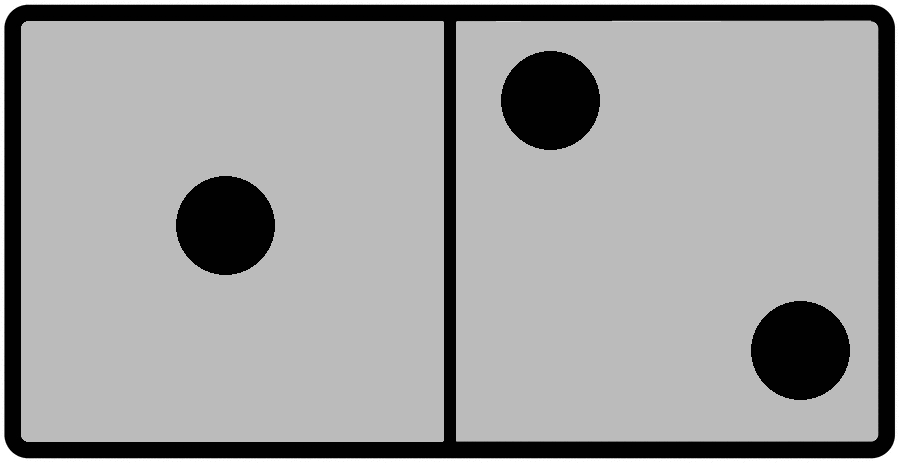
\includegraphics[width=0.07\textwidth]{gray1_2.png}}
and
\raisebox{-0.25\height}{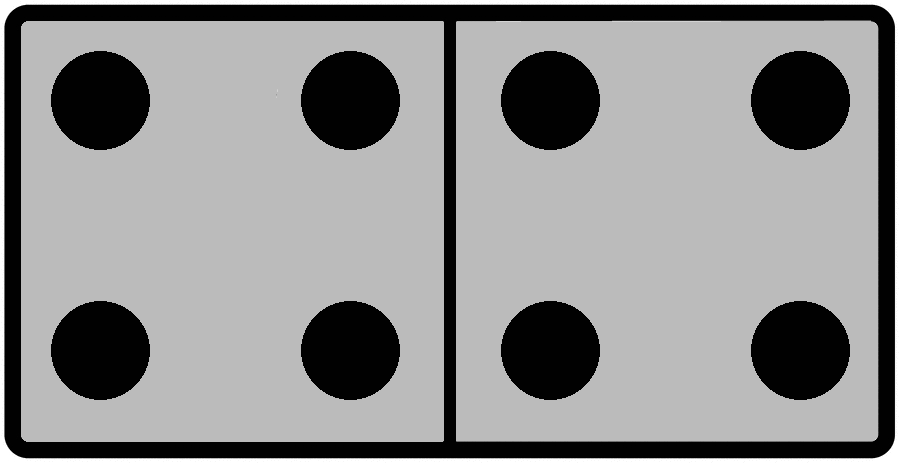
\includegraphics[width=0.07\textwidth]{gray4_4.png}} in
it, so $B_d = \{ [\ 1\ \ 2\ ], [\ 4\ \ 4\ ] \}$.)

We can translate between the two bases using matrix-vector multiplication. To
go from domino to standard, we merely put the dominoes into the columns of a
matrix:

\vspace{-.15in}
\begin{align*}
\textrm{COB}_{B_d \rightarrow B_s} =
\begin{bmatrix}
1 & 4 \\
2 & 4 \\
\end{bmatrix}
\end{align*}
\vspace{-.15in}

because

\vspace{-.15in}
\begin{align*}
\overrightarrow{r_{B_s}} =
\begin{bmatrix}
1 & 4 \\
2 & 4 \\
\end{bmatrix} \cdot
\overrightarrow{r_{B_d}} =
\begin{bmatrix}
1 & 4 \\
2 & 4 \\
\end{bmatrix} \cdot
\begin{bmatrix} 3 \\ -1 \end{bmatrix}_{B_d} =
\begin{bmatrix} -1 \\ 2 \end{bmatrix}_{B_s}.
\end{align*}
\vspace{-.15in}

This $\textrm{COB}_{B_d \rightarrow B_s}$ matrix is called the
\textbf{change-of-basis matrix} from the domino basis to the standard basis.

\bigskip
\index{Hermione}
\label{changeOfBasisOtherWayCliffhanger}

What if we want to go in the other direction? Remember, Hermione had a vector
$\overrightarrow{\textbf{h}}$ which, when expressed in the standard basis, was
{\scriptsize $\begin{bmatrix} 5 \\ 2 \end{bmatrix}$}. What are her coordinates
in the domino basis?

\index{inverse}
\smallskip

Hate to still leave you hanging on Hermione, but for that, we'll need a new
concept called the \textbf{matrix inverse}, which we won't get to until
p.~\pageref{matrixInverse}. Stay tuned.


\section{``Special'' matrices}

Finally, there are some terms for ``special'' matrices that satisfy certain
properties, which will come up for us in important contexts. We'll start with
the least restrictive definition and repeatedly add further constraints to it
for successively more restrictive ones.

\index{square matrix}
Easiest of all, a \textbf{square} matrix is simply one that has the same number
of rows and columns. Any $4\times 4$ matrix is square, and no $6\times 7$
matrix is square. Simple. And yes, in case you're wondering, we can have a
$1\times 1$ matrix, which is considered square.

\index{symmetric matrix}

In order for a matrix to be \textbf{symmetric}, it has to be
square.\footnote{There are more advanced versions of some of the definitions in
this section that don't require square-ness, but they won't come up for us.}
Further, in a symmetric matrix \textit{the rows and the columns are
interchangeable.} For example:

\vspace{-.15in}
\begin{align*}
\begin{bmatrix}
9 & 7 & 2 & 8\\
7 & -3 & 0 & -1\\
2 & 0 & 5 & 4 \\
8 & -1 & 4 & 16 \\
\end{bmatrix}
\end{align*}
\vspace{-.15in}

In this matrix, row \#0 is $[\ 9\ \ 7\ \ 2\ \ 8\ ]$, and column \#0 is
\textit{also} $[\ 9\ \ 7\ \ 2\ \ 8\ ]$. Similarly, row \#1 and column \#1 are
the same, as are row \#2 and column \#2, and row \#3 and column \#3.

\label{symmetric}

Mathematically, a matrix $M$ is symmetric only if:

\vspace{-.15in}
\begin{align*}
\forall i,j \ M_{i,j} = M_{j,i}.
\end{align*}
\vspace{-.15in}

In other words, you must be able to swap the row and column numbers and get the
same value. The entry at row 5 column 8 must be the same as the one at row 8
column 5, \textit{etc.} If that's not true every time, it's not a symmetric
matrix.

It might help you understand the meaning of ``symmetric'' if you mentally
visualize a line from the upper-left entry to the lower-right entry of the
matrix:

\vspace{-.15in}
\begin{align*}
\begin{bmatrix} \tikzmark{a}
9 & 7 & 2 & 8\\
7 & -3 & 0 & -1\\
2 & 0 & 5 & 4 \\
8 & -1 & 4 & 16 \tikzmark{b} \\
\end{bmatrix}
\end{align*}
\MyLine[thick]{a}{b}
\vspace{-.15in}

\index{main diagonal, of a matrix}
\index{diagonal, of a matrix}
\index{mirror}

These entries, by the way, where the row number equals the column number, are
called the \textbf{main diagonal} (or just the \textbf{diagonal}) of the
matrix. If a matrix is symmetric, you could imagine that line being a mirror:
and it perfectly reflects one side to the other. The two 7's are on matching,
opposite sides of that line, as are the two 2's, the two 0's, the two 8's, the
two $-1$'s, and the two 4's. Note that the entries \textit{on} the main
diagonal can be anything at all -- they don't affect the symmetric-ness (or
not) of the matrix.

This property may seem obscure, but it will come up surprisingly often.

By the way, you might have expected a ``symmetric matrix'' to be one that was a
mirror image of itself left-to-right-wise, or top-to-bottom-wise. Nope. That
doesn't turn out to be a useful concept. The definition above, however --
reflection along the main diagonal -- turns out to be immensely useful.

\medskip

\index{upper-triangular}
Okay, next one. A matrix is said to be \textbf{upper-triangular} if \textit{all
entries below the main diagonal are zero.} Example:

\vspace{-.15in}
\begin{align*}
\begin{bmatrix}
9 & 7 & 2 & 8\\
0 & -3 & 0 & -1\\
0 & 0 & 5 & 4 \\
0 & 0 & 0 & 16 \\
\end{bmatrix}
\end{align*}
\vspace{-.15in}

This matrix is upper-triangular because I've zeroed-out everything below the
$9,-3,5,16$ entries of the main diagonal. Note that it's perfectly fine to also
have a 0 above -- or even on -- the diagonal. The existence of such a zero
doesn't disqualify you from upper-triangular-ness. The only requirement is that
all entries \textit{below} the diagonal must be zero.

\index{lower-triangular}

You can probably tell why the word ``triangular'' is used: the possibly-nonzero
entries are all arranged in a right triangle in the upper-right half of the
matrix. Occasionally it will also be useful to talk about a
\textbf{lower-triangular} matrix, which has zeroes in every entry
\textit{above} the diagonal. And again, you have to be square for your upper-
or lower- triangular-ness to even be under consideration.

\medskip

\index{diagonal matrix}

Also common is the notion of a \textbf{diagonal matrix}. Be careful: a ``a
diagonal matrix'' is different from ``the diagonal \textit{of} a matrix!'' A
diagonal matrix is one where all entries \textit{not} on the diagonal must be
zero. Example:

\vspace{-.15in}
\begin{align*}
\begin{bmatrix}
9 & 0 & 0 & 0\\
0 & -3 & 0 & 0\\
0 & 0 & 5 & 0 \\
0 & 0 & 0 & 16 \\
\end{bmatrix}
\end{align*}
\vspace{-.15in}

Food for thought: a diagonal matrix is both upper-triangular \textit{and}
lower-triangular.

Like I said, we're getting more and more restrictive as we go. If you're
planning on being a $6\times 6$ diagonal matrix, there's a whole lot of your
life already set in stone. The only choices you have are what to put on your
diagonal.

\medskip

\index{identity matrix}
\label{identityMatrix}

But we can get more restrictive still! Believe it or not, a very common and
interesting type of matrix will be a so-called \textbf{identity matrix}. Get
this: an identity matrix is a diagonal matrix \textit{with only 1's on the
diagonal.} Talk about confining. Once you've decided on your size, you have
literally no choices. The one and only $4\times 4$ identity matrix is this one:

\vspace{-.15in}
\begin{align*}
\begin{bmatrix}
1 & 0 & 0 & 0\\
0 & 1 & 0 & 0\\
0 & 0 & 1 & 0 \\
0 & 0 & 0 & 1 \\
\end{bmatrix}
\end{align*}
\vspace{-.15in}

For every natural number $n$, there's one and only one identity matrix of that
size. Sometimes we call that matrix $I_n$ for short; in other words, the matrix
above is sometimes called $I_4$. 

In the next chapter (p.~\pageref{identityMatrixExplanation}, to be exact),
you'll learn the excellent reason that this kind of matrix is called an
``identity'' matrix. For now, test yourself with these questions:

\begin{compactenum}
\label{specialMatrixQuiz}
\item Are all square matrices symmetric?
\item Are all symmetric matrices square?
\item Are all symmetric matrices upper-triangular?
\item Are all upper-triangular matrices symmetric?
\item Are all diagonal matrices upper-triangular?
\item Are all upper-triangular matrices diagonal?
\item Are all diagonal matrices symmetric?
\item Are all diagonal matrices identity matrices?
\item Are all identity matrices upper-triangular?
\item Are all identity matrices diagonal?
\end{compactenum}

The answers are at the end of the chapter (p.~\pageref{specialMatrixQuizSols}).

\bigskip

\index{block diagonal matrix}

Rounding out our list, I'll mention two more types of ``special'' matrices that
are a bit different from the previous ones. The first is called a \textbf{block
diagonal matrix}. A matrix is block diagonal if it can be partitioned into
rectangular chunks (called ``blocks'') such that each chunk on the diagonal is
square, and all entries in the non-diagonal chunks must be all zeros.

Whoa, that's hard to visualize. Let's look at some examples:

\vspace{-.15in}
\begin{align*}
\mleft[
\begin{array}{cccc}
3 & 2 & 0 & 0\\
4 & 4 & 0 & 0\\
0 & 0 & 9 & 7 \\
0 & 0 & 2 & 6 \\
\end{array}
\mright]
\end{align*}
\vspace{-.15in}

This is a block diagonal matrix. Why? Because if we break it up this way:

\vspace{-.15in}
\begin{align*}
\mleft[
\begin{array}{cc|cc}
3 & 2 & 0 & 0\\
4 & 4 & 0 & 0\\
\hline
0 & 0 & 9 & 7 \\
0 & 0 & 2 & 6 \\
\end{array}
\mright]
\end{align*}
\vspace{-.15in}

we can see that it satisfies the conditions. The two blocks on the diagonal
(which are the 3--2--4--4 block and the 9--7--2--6 block) are square ($2\times
2$), and all the entries in the off-diagonal blocks are zeroes.

Sometimes it can take a little fiddling around to find the right partition. Try
this one:
\pagebreak
\begin{align*}
\mleft[
\begin{array}{cccc}
1 & 4 & 3 & 0\\
6 & 8 & 2 & 0\\
5 & 1 & 5 & 0 \\
0 & 0 & 0 & 7 \\
\end{array}
\mright]
\end{align*}
\vspace{-.15in}

Does that one look block diagonal to you? It is:

\vspace{-.15in}
\begin{align*}
\mleft[
\begin{array}{ccc|c}
1 & 4 & 3 & 0\\
6 & 8 & 2 & 0\\
5 & 1 & 5 & 0 \\
\hline
0 & 0 & 0 & 7 \\
\end{array}
\mright]
\end{align*}
\vspace{-.15in}

Notice that the blocks that are \textit{not} on the diagonal don't have to be
square. All that matters are the diagonal blocks, and here we have a $3\times
3$ and a $1\times 1$, so we're good.

Here's one more for the road:

\vspace{-.15in}
\begin{align*}
\mleft[
\begin{array}{ccccccc}
4 & 0 & 0 & 0 & 0 & 0 & 0\\
0 & 9 & 0 & 3 & 3 & 0 & 0\\
0 & 0 & 0 & 0 & 0 & 0 & 0\\
0 & 0 & 2 & 0 & 0 & 0 & 0\\
0 & 7 & 0 & 0 & 5 & 0 & 0\\
0 & 0 & 0 & 0 & 0 & 6 & 3\\
0 & 0 & 0 & 0 & 0 & 1 & 0\\
\end{array}
\mright]
\end{align*}
\vspace{-.15in}

Is this one, too, block diagonal? All the extra (and unnecessary) zeroes might
fool you, but if you partition it this way:

\vspace{-.15in}
\begin{align*}
\mleft[
\begin{array}{c|cccc|cc}
4 & 0 & 0 & 0 & 0 & 0 & 0\\
\hline
0 & 9 & 0 & 3 & 3 & 0 & 0\\
0 & 0 & 0 & 0 & 0 & 0 & 0\\
0 & 0 & 2 & 0 & 0 & 0 & 0\\
0 & 7 & 0 & 0 & 5 & 0 & 0\\
\hline
0 & 0 & 0 & 0 & 0 & 6 & 3\\
0 & 0 & 0 & 0 & 0 & 1 & 0\\
\end{array}
\mright]
\end{align*}
\vspace{-.15in}

you can see that it is.

\bigskip

\index{orthogonal}
\index{orthogonal matrix}

Finally finally, let me introduce the concept of an ``\textbf{orthogonal}
matrix.'' A matrix must meet two criteria in order to deserve the title
``orthogonal'':

\label{orthogonalMatrices}

\begin{compactenum}
\itemsep.1em

\item Each of its \textit{columns} must be orthogonal to each of the other
columns. (Recall from p.~\pageref{orthogonalMeansZeroDotProduct} that two
vectors are orthogonal if their dot product is zero.)

\item The (Euclidean) norm of each of its columns must be equal to 1. (Recall
that to compute the Euclidean norm of a vector, you just take the
square-root-of-the-sum-of-its-elements-squared, a.k.a. the Pythagorean Theorem.
See p.~\pageref{Euclideannorm}.)

\end{compactenum}

Okay, that seemed kind of random. But it actually has important implications,
which will come up later in the book. For now, let me just show some examples
of each:

\vspace{-.15in}
\begingroup
\renewcommand*{\arraystretch}{1.5}
\begin{align*}
A =
\begin{bmatrix}
2 & 1 \\
-2 & 1 \\
\end{bmatrix},\quad
B =
\begin{bmatrix}
\frac{\sqrt{2}}{2} & 1 \\
\frac{\sqrt{2}}{2} & 0 \\
\end{bmatrix},\quad
C =
\begin{bmatrix}
\frac{2}{5} & \frac{3}{5} \\
\frac{3}{5} & -\frac{2}{5} \\
\end{bmatrix},\quad
D =
\begin{bmatrix}
1 & 0 \\
0 & 1 \\
\end{bmatrix}.
\end{align*}
\endgroup

\smallskip
Question: which of these matrices are orthogonal? Answers:

\vspace{-.1in}
\begin{itemize}
\itemsep.9em

\item $A$ is \textit{not}. It passes the first criterion, since
${\scriptsize \begin{bmatrix} 2 \\ -1 \end{bmatrix}} \cdot
{\scriptsize \begin{bmatrix} 1 \\ 1 \end{bmatrix}}$ does equal zero (check my
math!) but the two columns don't have Euclidean length 1. (The norm of the
left column for instance, is $\sqrt{2^2 + (-2)^2} = 2.828\dots$) Next!

\item $B$ is \textit{not}. It passes the second criterion (the Euclidean norms of both
columns are 0 -- double-check that) but not the first, since the dot product of
the two columns is $\frac{\sqrt{2}}{2} = .707\dots$ (Double-check that, too.)
Next!

\item Matrix $C$, on the other hand, \textit{is} orthogonal. The dot product of
its two columns is zero:

\vspace{-.15in}
\begin{align*}
\frac{2}{5} \cdot \frac{3}{5} + 
\frac{3}{5} \cdot \Big(-\frac{2}{5}\Big) = \frac{6}{25} - \frac{6}{25} = 0,
\end{align*}
\vspace{-.15in}

and each column has norm 1:

\vspace{-.15in}
\begin{align*}
\Bigg(\sqrt{\frac{2}{5}}\Bigg)^2 &+ \Bigg(\sqrt{\frac{3}{5}}\Bigg)^2 = 1,
\textrm{and} \\
\Bigg(\sqrt{\frac{3}{5}}\Bigg)^2 &+ \Bigg(-\sqrt{\frac{2}{5}}\Bigg)^2 = 1.
\end{align*}
\vspace{-.15in}

Yay!

\item And lastly, realize that the identity matrix $D$ is also orthogonal! Both
criteria are satisfied by inspection. This is true of any identity matrix,
you'll realize as soon as you consider it.

\end{itemize}

\index{orthonormal}

I haven't yet told you why orthogonal matrices are important, but we'll return
to this in future chapters.

\index{King of the World}
\index{Stephen, King of the World}

By the way, if I were King of the World, I wouldn't have called these
``orthogonal matrices.'' I would have called them ``\textbf{orthonormal}
matrices.'' That's because two vectors which are both perpendicular to each
other (with zero dot product, and therefore orthogonal) \textit{and} which also
each have Euclidean norm 1 (and thus are ``normalized'' in length) are called
\textbf{orthonormal vectors}.

When I'm King, I'll redefine these terms so that ``orthogonal matrix'' means
any matrix that satisfies criterion \#1, above (but not necessarily \#2), and
reserve the new term ``orthonormal matrix'' for any matrix that satisfies
\textit{both} criteria. Until then, we'll have to keep using the misleading
term ``orthogonal matrix.'' (Keep a watch on your news feed for that
Stephen-becomes-King-of-the-World thing -- I'm still working on it.)

\vspace{.1in}
\hrulefill \\

\pagebreak

\section*{\faPython \ \ \textit{Appendix: Python}}

\index{array}
\index{ndarray@\texttt{ndarray} (NumPy type)}
\index{NumPy}

\index{index number}
\index{dimension}

With NumPy, a matrix is very similar to a vector. That's because they're both
\texttt{ndarray}s. They only vary in the number of \textbf{dimensions}, but we
have to be careful here because NumPy uses the term ``dimension'' in a
different way than we've been doing (say, on p.~\pageref{dimension}). In our
lingo, a matrix with three rows and four columns has dimensions $3\times 4$.
But NumPy would say that this matrix -- and \textit{all} matrices -- has
dimension \textbf{2}. Why 2? Because it has a left-to-right dimension (rows)
and an up-and-down dimension (columns).

\index{tensor}

For us, this won't be too complicated, because we won't be dealing with objects
of higher dimension (which are called \textbf{tensors}, by the way) than 2. So
all this really means for us is that a one-dimensional \texttt{ndarray} is a
vector, and a two-dimensional \texttt{ndarray} is a matrix. And when we want to
zero in on a particular element of a matrix, we need \textit{two} index
numbers: one for the row and one for the column.

\subsection*{Creating matrices (2-d arrays)}

\index{[]@\texttt{[]} (boxies)}
\index{boxies (square brackets)}

Creating a NumPy matrix is a snap -- you just need to be prepared to type a lot
of boxies. Here's a $3\times 2$ matrix:

\begin{Verbatim}[fontsize=\small,samepage=true,frame=single,framesep=3mm]
mat = array([[6,9],[4,5],[1,4]])
\end{Verbatim}
\vspace{-.2in}

Notice the boxies-within-boxies: the very outermost pair is for the entire
array, where each inner pair specifies one row. In this way, you see that a
matrix is an array-of-arrays; or, if you prefer, a list of rows. We can print
them the same way we did vectors:

\begin{Verbatim}[fontsize=\small,samepage=true,frame=single,framesep=3mm]
print(mat)
\end{Verbatim}
\vspace{-.2in}

\begin{Verbatim}[fontsize=\small,samepage=true,frame=leftline,framesep=5mm,framerule=1mm]
[[6 9]
 [4 5]
 [7 4]]
\end{Verbatim}

\medskip
\index{zeros@\texttt{zeros()} function}

The \texttt{zeros()} function works for matrices, but with a slightly different
syntax: we specify the dimensions we'd like after the word \texttt{shape} and a
comma:

\begin{Verbatim}[fontsize=\small,samepage=true,frame=single,framesep=3mm]
nada = zeros(shape=(4,7))
print(nada)
\end{Verbatim}
\vspace{-.2in}

\begin{Verbatim}[fontsize=\small,samepage=true,frame=leftline,framesep=5mm,framerule=1mm]
[[0. 0. 0. 0. 0. 0. 0.]
 [0. 0. 0. 0. 0. 0. 0.]
 [0. 0. 0. 0. 0. 0. 0.]
 [0. 0. 0. 0. 0. 0. 0.]]
\end{Verbatim}

\medskip
\index{random@\texttt{random.rand()} function}

And we can do the random number thing, too, by passing the
\texttt{random.rand()} function dimension numbers:

\begin{Verbatim}[fontsize=\small,samepage=true,frame=single,framesep=3mm]
crazy = random.rand(3,5)
print(crazy)
\end{Verbatim}
\vspace{-.2in}

\begin{Verbatim}[fontsize=\small,samepage=true,frame=leftline,framesep=5mm,framerule=1mm]
[[0.09121684 0.3084825  0.2529024  0.78089448 0.46138631]
 [0.30003058 0.9275848  0.72649169 0.10995998 0.97565467]
 [0.32876047 0.25447349 0.78955441 0.07921066 0.20986057]]
\end{Verbatim}

(As before, each number is between 0 and 1.)

\medskip
\index{loadtxt@\texttt{loadtxt()} (NumPy)}
\index{plain-text file}
\index{txt file@\texttt{.txt} file}

Lastly, we can read a matrix from a file just like we did with a vector. Most
commonly, such files will use a comma as a \textbf{delimiter} to separate
entries on a line, so we'll specify that in our function call:

\begin{Verbatim}[fontsize=\small,samepage=true,frame=single,framesep=3mm]
my_matrix = loadtxt("somematrixdata.txt", delimiter=",")
\end{Verbatim}

\index{csv file@\texttt{.csv} file}
\index{csv@CSV (comma-separated values)}

By the way, often files like these will have a \texttt{.csv} extension instead
of \texttt{.txt}; this stands for \textbf{comma-separated values}, for obvious
reasons.


\subsection*{Working with matrices (arrays)}

index{shape@\texttt{.shape}}

To learn the dimensions of a matrix, use \texttt{.shape} which gives a vector
of the dimensions:

\begin{Verbatim}[fontsize=\small,samepage=true,frame=single,framesep=3mm]
print(mat)
print(mat.shape)
print("The matrix has {} rows.".format(mat.shape[0]))
print("The matrix has {} columns.".format(mat.shape[1]))
\end{Verbatim}
\vspace{-.2in}

\begin{Verbatim}[fontsize=\small,samepage=true,frame=leftline,framesep=5mm,framerule=1mm]
[[6 9]
 [4 5]
 [1 4]]
(3, 2)
The matrix has 3 rows.
The matrix has 2 columns.
\end{Verbatim}


We can give a matrix \textit{two} index numbers (comma-separated) to retrieve
or change individual elements:

\begin{Verbatim}[fontsize=\small,samepage=true,frame=single,framesep=3mm]
print(mat[0,1])
print(mat[2,0])
mat[1,1] = 19
print(mat)
\end{Verbatim}
\vspace{-.2in}

\begin{Verbatim}[fontsize=\small,samepage=true,frame=leftline,framesep=5mm,framerule=1mm]
2
7
[[ 3  2]
 [ 4 19]
 [ 7  4]]
\end{Verbatim}

\index{:@\texttt{:} (colon)}
\index{colon operator (NumPy)}

Note that both rows and columns are indexed starting at 0.

\medskip

We can get an entire row, or an entire column, by using a colon
(``\texttt{:}'') in place of one of the indices:

\begin{Verbatim}[fontsize=\small,samepage=true,frame=single,framesep=3mm]
print(mat[2,:])
print(mat[:,1])
\end{Verbatim}
\vspace{-.2in}

\begin{Verbatim}[fontsize=\small,samepage=true,frame=leftline,framesep=5mm,framerule=1mm]
[1 4]
[ 9 19  4]
\end{Verbatim}

Somewhat weirdly, getting exactly one column (as we did in the second operation
just now) gives us back the correct (column) vector, but instead of printing it
out as a column, NumPy prints it as a row. Trying to save screen space? Not
sure.

\index{slice}
\medskip

Our slicing technique works the same as before (p.~\pageref{slice}), on the
rows and/or the columns. Let's create a slightly bigger matrix to show it off:

\begin{Verbatim}[fontsize=\small,samepage=true,frame=single,framesep=3mm]
bigger = array([[-9,-8,-7],[2,4,-6],[0,0,0],[1,9,6]])
print(bigger)
\end{Verbatim}
\vspace{-.2in}
\begin{Verbatim}[fontsize=\small,samepage=true,frame=leftline,framesep=5mm,framerule=1mm]
[[-9 -8 -7]
 [ 2  4 -6]
 [ 0  0  0]
 [ 1  9  6]]
\end{Verbatim}

\begin{Verbatim}[fontsize=\small,samepage=true,frame=single,framesep=3mm]
print(bigger[1,0:2])
\end{Verbatim}
\vspace{-.2in}

\begin{Verbatim}[fontsize=\small,samepage=true,frame=leftline,framesep=5mm,framerule=1mm]
[2 4]
\end{Verbatim}

\begin{Verbatim}[fontsize=\small,samepage=true,frame=single,framesep=3mm]
print(bigger[0:3,1:3])
\end{Verbatim}
\vspace{-.2in}

\begin{Verbatim}[fontsize=\small,samepage=true,frame=leftline,framesep=5mm,framerule=1mm]
[[-8 -7]
 [ 4 -6]
 [ 0  0]]
\end{Verbatim}

\begin{Verbatim}[fontsize=\small,samepage=true,frame=single,framesep=3mm]
print(bigger[0:3,2])
\end{Verbatim}
\vspace{-.2in}

\begin{Verbatim}[fontsize=\small,samepage=true,frame=leftline,framesep=5mm,framerule=1mm]
[-7 -6  0]
\end{Verbatim}

(Yeah, displays as row vector, it's weird I agree.)

\medskip
\index{transpose@\texttt{.transpose()}}

Finally, some linear algebra operations. We can take the transpose of a matrix
by appending \texttt{.transpose()}:

\begin{Verbatim}[fontsize=\small,samepage=true,frame=single,framesep=3mm]
print(bigger.transpose())
\end{Verbatim}
\vspace{-.2in}

\begin{Verbatim}[fontsize=\small,samepage=true,frame=leftline,framesep=5mm,framerule=1mm]
[[-9  2  0  1]
 [-8  4  0  9]
 [-7 -6  0  6]]
\end{Verbatim}

\index{matrix-vector multiplication}
\index{dot@\texttt{.dot()}}

And matrix-vector multiplication also uses the \texttt{.dot()} syntax:

\begin{Verbatim}[fontsize=\small,samepage=true,frame=single,framesep=3mm]
x = array([4,5,6])
print(bigger.dot(x))
\end{Verbatim}
\vspace{-.2in}

\begin{Verbatim}[fontsize=\small,samepage=true,frame=leftline,framesep=5mm,framerule=1mm]
[-118   -8    0   85]
\end{Verbatim}


\subsection*{Python branching}

\index{branching}
\index{indentation (in Python)}
\index{if statement@\texttt{if} statement}

Finally, one more Python programming thing. Every programming language has ways
to \textbf{branch}, which means to control the flow of the program so that the
lines aren't executed in strict sequential order, depending on the situation.
Python uses the ``\texttt{if} statement'' for this, and again relies on
indentation to know where the relevant block of code ends. They are often used
in conjunction with \texttt{for} loops. Example:

\index{weights@\texttt{weights}}

\begin{Verbatim}[fontsize=\footnotesize,samepage=true,frame=single,framesep=3mm]
weights = np.array([ 145.6, 212.9, 126.4 ])

for i in arange(weights.size):
   if weights[i] < 150:
      print("You weigh {} lbs and might consider eating more."
         .format(weights[i]))
   print("Thanks for weighing in!")
\end{Verbatim}
\vspace{-.2in}

\begin{Verbatim}[fontsize=\small,samepage=true,frame=leftline,framesep=5mm,framerule=1mm]
You weigh 145.6 lbs and might consider eating more.
Thanks for weighing in!
Thanks for weighing in!
You weigh 126.4 lbs and might consider eating more.
Thanks for weighing in!
\end{Verbatim}

Each time the loop is executed, \texttt{i} has a different value, and hence the
next element of the \texttt{weights} vector is considered. Only if that
particular element satisfies the condition (less than 150) does the indented
code under the \texttt{if} get executed. Note that the ``\texttt{Thanks!}''
message gets printed out \textit{regardless} of the weight. Only lines indented
to the right of the \texttt{if} are what the \texttt{if} statement controls.

The ``\texttt{weights[i] < 150}'' part is called the \texttt{if} statement's
\textbf{condition}, and there is some wacky syntax you have to master to write
them correctly. Here it is:

\begin{center}
\begin{tabular}{c|c}
Operator & Meaning \\
\hline
\texttt{>} & greater than \\
\hline
\texttt{<} & less than \\
\hline
\texttt{>=} & greater than or equal to \\
\hline
\texttt{<=} & less than or equal to \\
\hline
\texttt{!=} & \textit{not} equal to \\
\hline
\texttt{==} & equal to \\
\hline
\texttt{and} & and \\
\hline
\texttt{or} & or \\
\hline
\texttt{not} & not \\
\end{tabular}
\end{center}

The last three of those are used when creating a \textbf{compound condition}
comprised of more than one test. For example:

\begin{Verbatim}[fontsize=\small,samepage=true,frame=single,framesep=3mm]
    if (sex[i] == "male" and weights[i] < 160  or
        sex[i] == "female" and weights[i] < 140):
        ...
\end{Verbatim}

Here, the body of the \texttt{if} statement will only be executed for males
under 160 lbs and for females under 140 lbs.

\subsection*{Boolean variables in Python}

The raw material that \texttt{if} statements work with is of the
\textbf{Boolean} type, not numbers, strings, or anything else. A Boolean
variable, named after 19th-century logician George Boole, holds either the
value \texttt{True} or \texttt{False}. (And these are capitalized in Python.)

It's common for a function to return a Boolean when its purpose is to check
whether some condition holds. Let's write a function called
\texttt{is\_square()} to determine whether a matrix is square. Here goes:

\index{is\_square@\texttt{is\_square()}}
\index{square matrix}
\index{return statement@\texttt{return} statement}
index{shape@\texttt{.shape}}

\label{multipleReturns}

\begin{Verbatim}[fontsize=\small,samepage=true,frame=single,framesep=3mm]
def is_square(m):
    if m.shape[0] == m.shape[1]:
        return True
    else:
        return False
\end{Verbatim}

\index{else@\texttt{else} branch}

Here we've added another feature to our \texttt{if} statement, namely an
\textbf{else branch}. I'm sure you can guess what it means, even if you've
never seen an \texttt{if}/\texttt{else} construction before: the code indented
under \texttt{else} gets executed \textit{only} if the condition in the
\texttt{if} statement is \texttt{False}. So an \texttt{if}/\texttt{else} is
simply an either/or.

You'll remember I mentioned in the last chapter that some functions have more
than one \texttt{return} statement in them. Now you can see why that would be
useful. A function finishes immediately as soon as it encounters a
\texttt{return}, and does not execute any code below it. However, because of
\texttt{if} statements, the path through a function might zigzag over and past
some \texttt{return} statements before reaching others.

Anyway, you can see how this function works: it simply compares the number of
rows in the matrix with the number of columns, and returns \texttt{True} if
these are the same. That, after all, is the definition of squareness.

\bigskip

\index{is\_diagonal@\texttt{is\_diagonal()}}
\index{diagonal matrix}
Here's another example:

\begin{Verbatim}[fontsize=\small,samepage=true,frame=single,framesep=3mm]
def is_diagonal(m):
    if m.shape[0] != m.shape[1]:
        return False
    for i in arange(m.shape[0]):
        for j in arange(m.shape[1]):
            if i != j  and  m[i,j] != 0:
                return False
    return True
\end{Verbatim}

That one packs a wallop. Can you figure out how it works?

First, we check to see if the matrix is square, since the way we've defined
diagonal matrices in this book, they must be square. If that check fails, we
immediately return our answer -- \texttt{False} -- and unpause our Netflix
video. If it \textit{is} square, however, we have more work to do.

\index{nested for loop@nested \texttt{for} loop}
\index{for loop@\texttt{for} loop}

The further work involves a \textbf{nested for loop}, since we need to examine
all elements of the matrix \texttt{m}: every row and every column. I have the
\texttt{i} loop variable going through the rows, and for \textit{each} row, the
\texttt{j} loop goes through all the columns. (It's important that you see how
each iteration of the outer (\texttt{i}) loop results in \textit{multiple}
iterations of the inner (\texttt{j}) loop.)

Now for every element, I check two things. First, does its row number equal its
column number? If these are equal, then that means the element I'm examining is
on the diagonal. Nothing special is required in this case; a diagonal matrix is
free to have anything it wants on its diagonal. However, if \texttt{i} does
\textit{not} equal \texttt{j}, then I'm examining an off-diagonal entry. If the
matrix in question is truly diagonal, all of those off-diagonal entries had
better be 0. As soon as I find an off-diagonal, non-zero entry, I immediately
raise my red flag and return from the function, again with a negative answer.

\index{else@\texttt{else} branch}

Only after I've gone through \textit{every} entry, and confirmed that
\textit{all} of the off-diagonal entries are zero, can I declare victory and
return \texttt{True}. Many students mess up on this part: they often put an
\texttt{else} branch on that \texttt{if}. This is fine syntactically, but wrong
logically: just because I find a single entry that satisfies my criteria does
not mean the entire matrix is therefore diagonal! No, I can only dare to return
\texttt{True} at the very, very end, after checking everything out.

Let's see whether our functions work. First, we'll create three matrices of
varying contents, and print them out:

\begin{Verbatim}[fontsize=\small,samepage=true,frame=single,framesep=3mm]
m1 = array([[2,3,4],[5,6,7]])
m2 = array([[5,0,1],[0,3,0],[0,0,9]])
m3 = array([[16,0,0],[0,27,0],[0,0,5]])
print(m1)
print(m2)
print(m3)
\end{Verbatim}
\vspace{-.2in}

\begin{Verbatim}[fontsize=\small,samepage=true,frame=leftline,framesep=5mm,framerule=1mm]
[[2 3 4]
 [5 6 7]]

[[5 0 1]
 [0 3 0]
 [0 0 9]]

[[16  0  0]
 [ 0 27  0]
 [ 0  0  5]]
\end{Verbatim}

Then, let's call both functions on each of them, and see which ones return
\texttt{True}:

\begin{Verbatim}[fontsize=\small,samepage=true,frame=single,framesep=3mm]
if is_square(m1):
    print("m1 is square!")
if is_diagonal(m1):
    print("m1 is diagonal!")
if is_diagonal(m2):
    print("m2 is diagonal!")
if is_square(m2):
    print("m2 is square!")
if is_square(m3):
    print("m3 is square!")
if is_diagonal(m3):
    print("m3 is diagonal!")
\end{Verbatim}
\vspace{-.2in}

\begin{Verbatim}[fontsize=\small,samepage=true,frame=leftline,framesep=5mm,framerule=1mm]
m2 is square!
m3 is square!
m3 is diagonal!
\end{Verbatim}

We hereby declare victory. 

\bigskip

Do you think you could write an \texttt{is\_upper\_triangular()} function in
this vein? \texttt{is\_symmetric()}? How about \texttt{is\_orthogonal()} or
\texttt{is\_block\_diagonal()}? Clearly, some of these are way harder than
others to write the code for, but all are indeed possible with Python.

\vspace{.4in}
\hrulefill \\

\subsection*{Answers to ``special'' matrix quiz from
p.~\pageref{specialMatrixQuiz}}

\label{specialMatrixQuizSols}

\begin{multicols}{3}
\begin{compactenum}
\item No.
\item Yes.
\item No.
\item No.
\item Yes.
\item No.
\item Yes.
\item No.
\item Yes.
\item Yes.
\end{compactenum}
\end{multicols}

